\chapter{Goal/Objectives}
\label{ch:goal} % This how you label a chapter and the key (e.g., ch:into) will be used to refer this chapter ``Introduction'' later in the report. 
% the key ``ch:into'' can be used with command \ref{ch:intor} to refere this Chapter.
\section{Goals of this project:}
\begin{itemize}
    \item Implement a multi-agent system that includes different levels of intelligence for a card-playing bot.
    \item Define and implement autonomous behaviors for the bots, allowing them to make strategic decisions based on the context of the game.
    \begin{itemize}
        \item Casual player
        \item Make an HiLo strategic agent.
        \item Create a group of strategic agents that suggest moves to the player.
    \end{itemize}
    \item Transpose agent decision on a GUI that shows a visual table and cards.
    \item Measure the winning rate of the agents.
\end{itemize}

\section{Usage scenarios}

Smart 21 will be a full simulation of the real game. Users can decide to play 21 for fun or test the ability of the agents by letting them play and analyze their stategies.  

\section{Definition of done}

Final delivery will be a gradle project that has different running options:

\begin{itemize}
    \item 1. Pure 21 game.
    \item 2. Dumb agent that plays with BDI defined by common sense.
    \item 3. HiLo agent that expoilts HiLO algorithm to count cards and decide autonomously how much money bet on a hand.
    \item 4. Consensuos guided agent by different strategies.
\end{itemize}

To test the agents implementation will be measured the amount of money won and risked and compared this data in a grafical representation.

\chapter{Background and link to the theory}

(To be written at the end)
• Relevant architectural styles (the ones mentioned in Section 3)
• Relevant interaction patterns (the ones mentioned in Section 3)
• Relevant software frameworks (the ones mentioned in Sections 3 and 4)

\textbf{Blackjack} is a popular casino card game where players compete against the dealer to get a score as close as possible to \textbf{21} without exceeding it. It is a game of skill, strategy, and luck, widely played in both physical and online casinos.

\section{Basic Rules}

\begin{itemize}
    \item The game is played with one or more decks of \textbf{52 cards}.
    \item Numbered cards (2-10) have their face value, face cards (J, Q, K) are worth \textbf{10}, and the Ace can be worth \textbf{1 or 11}, depending on what benefits the player.
    \item Each player and the dealer receive \textbf{two initial cards}. The dealer reveals one of their cards.
    \item The player can decide to:
    \begin{itemize}
        \item \textbf{Hit} -- draw another card.
        \item \textbf{Stand} -- keep the current hand.
        \item \textbf{Double Down} -- double the bet and receive only one more card.
        \item \textbf{Split} -- if holding a pair, the player can split them into two separate hands.
    \end{itemize}
\end{itemize}

\section{Objective of the Game}

\begin{itemize}
    \item The goal is to have a score \textbf{closer to 21} than the dealer without exceeding it.
    \item If the score exceeds \textbf{21}, the player loses immediately (\textit{bust}).
    \item If the dealer exceeds 21, all remaining players win.
\end{itemize}

\section{Dealer's Rules}

\begin{itemize}
    \item The dealer must \textbf{draw cards until reaching 16}.
    \item The dealer must \textbf{stand on 17 or higher}.
\end{itemize}

\section{Winning and Payouts}

\begin{itemize}
    \item If the player beats the dealer, they win an amount equal to their bet.
    \item If the player gets a \textbf{natural Blackjack} (Ace + 10 or face card), they win \textbf{1.5 times} their bet.
    \item If the player and dealer have the same score, the bet is returned (\textit{Push}).
\end{itemize}

Blackjack is a game that combines luck and strategy, with optimal strategy charts to maximize winning chances. Would you like some tips on basic strategy?


//TODO inserire alcuni screen di gioco 


\chapter{Requirements Analysis}

\section{Implicit Requirements}
\begin{itemize}
   \item Software must adhere to the rules of 21, so it must be capable of know who wins the hand and give the right amount of money to the winner.
   \item Users must be capable of following the game flow so the agents need to implement a slowdown mechanism and maybe a clear log.
   \item During each phase of the game the agent must know what to do from his understandings.
   \item Bots should exhibit appropriate strategic behaviors based on their level and knowledge about the game.
\end{itemize}

\chapter{Design}

This is a multi-purpose system, it can be used as a classical game to occupy time by a user or can be played by intelligent agent to instruct the user with some basic stategy of the game. \textbf{MAS (Multi-agent-system)} architecture is used here to coordinate the activities of the player agents and strategic agents. A good abstraction used is the one that compares the Environment typically used in MAS with the table game where agents, based on their intentions and belief react according to changes like: 
\begin{itemize}
    \item Place the cards.
    \item Stand.
    \item Bet.
    \item Raise the bet.
    \item Every entity involved in the action can perfectly see the (virtual) table with cards and money on
 \end{itemize}

The interaction between agents is controlled by \textbf{TwentyOneEnvironment} that encapsulates a gameTable object that contains most of the business logic of the game. This system includes also a user graphical interface for monitoring the developement of the game.

\section{Structure (domain entities)}

\begin{table}[h]
    \centering
    \renewcommand{\arraystretch}{1.3}
    \begin{tabular}{|c|p{8cm}|}
        \hline
        \textbf{Entity} & \textbf{Description} \\
        \hline
        Player & The main participant who makes decisions based on game conditions. \\
        \hline
        Dealer & The entity responsible for managing the game, distributing cards, and enforcing rules. \\
        \hline
        Strategic Agent & An abstract entity that provides advice to the player and influences their decisions. \\
        \hline
    \end{tabular}
    \caption{Domain Entities}
    \label{tab:domain_entities}
\end{table}

\begin{figure}[!htb]
    \centering
    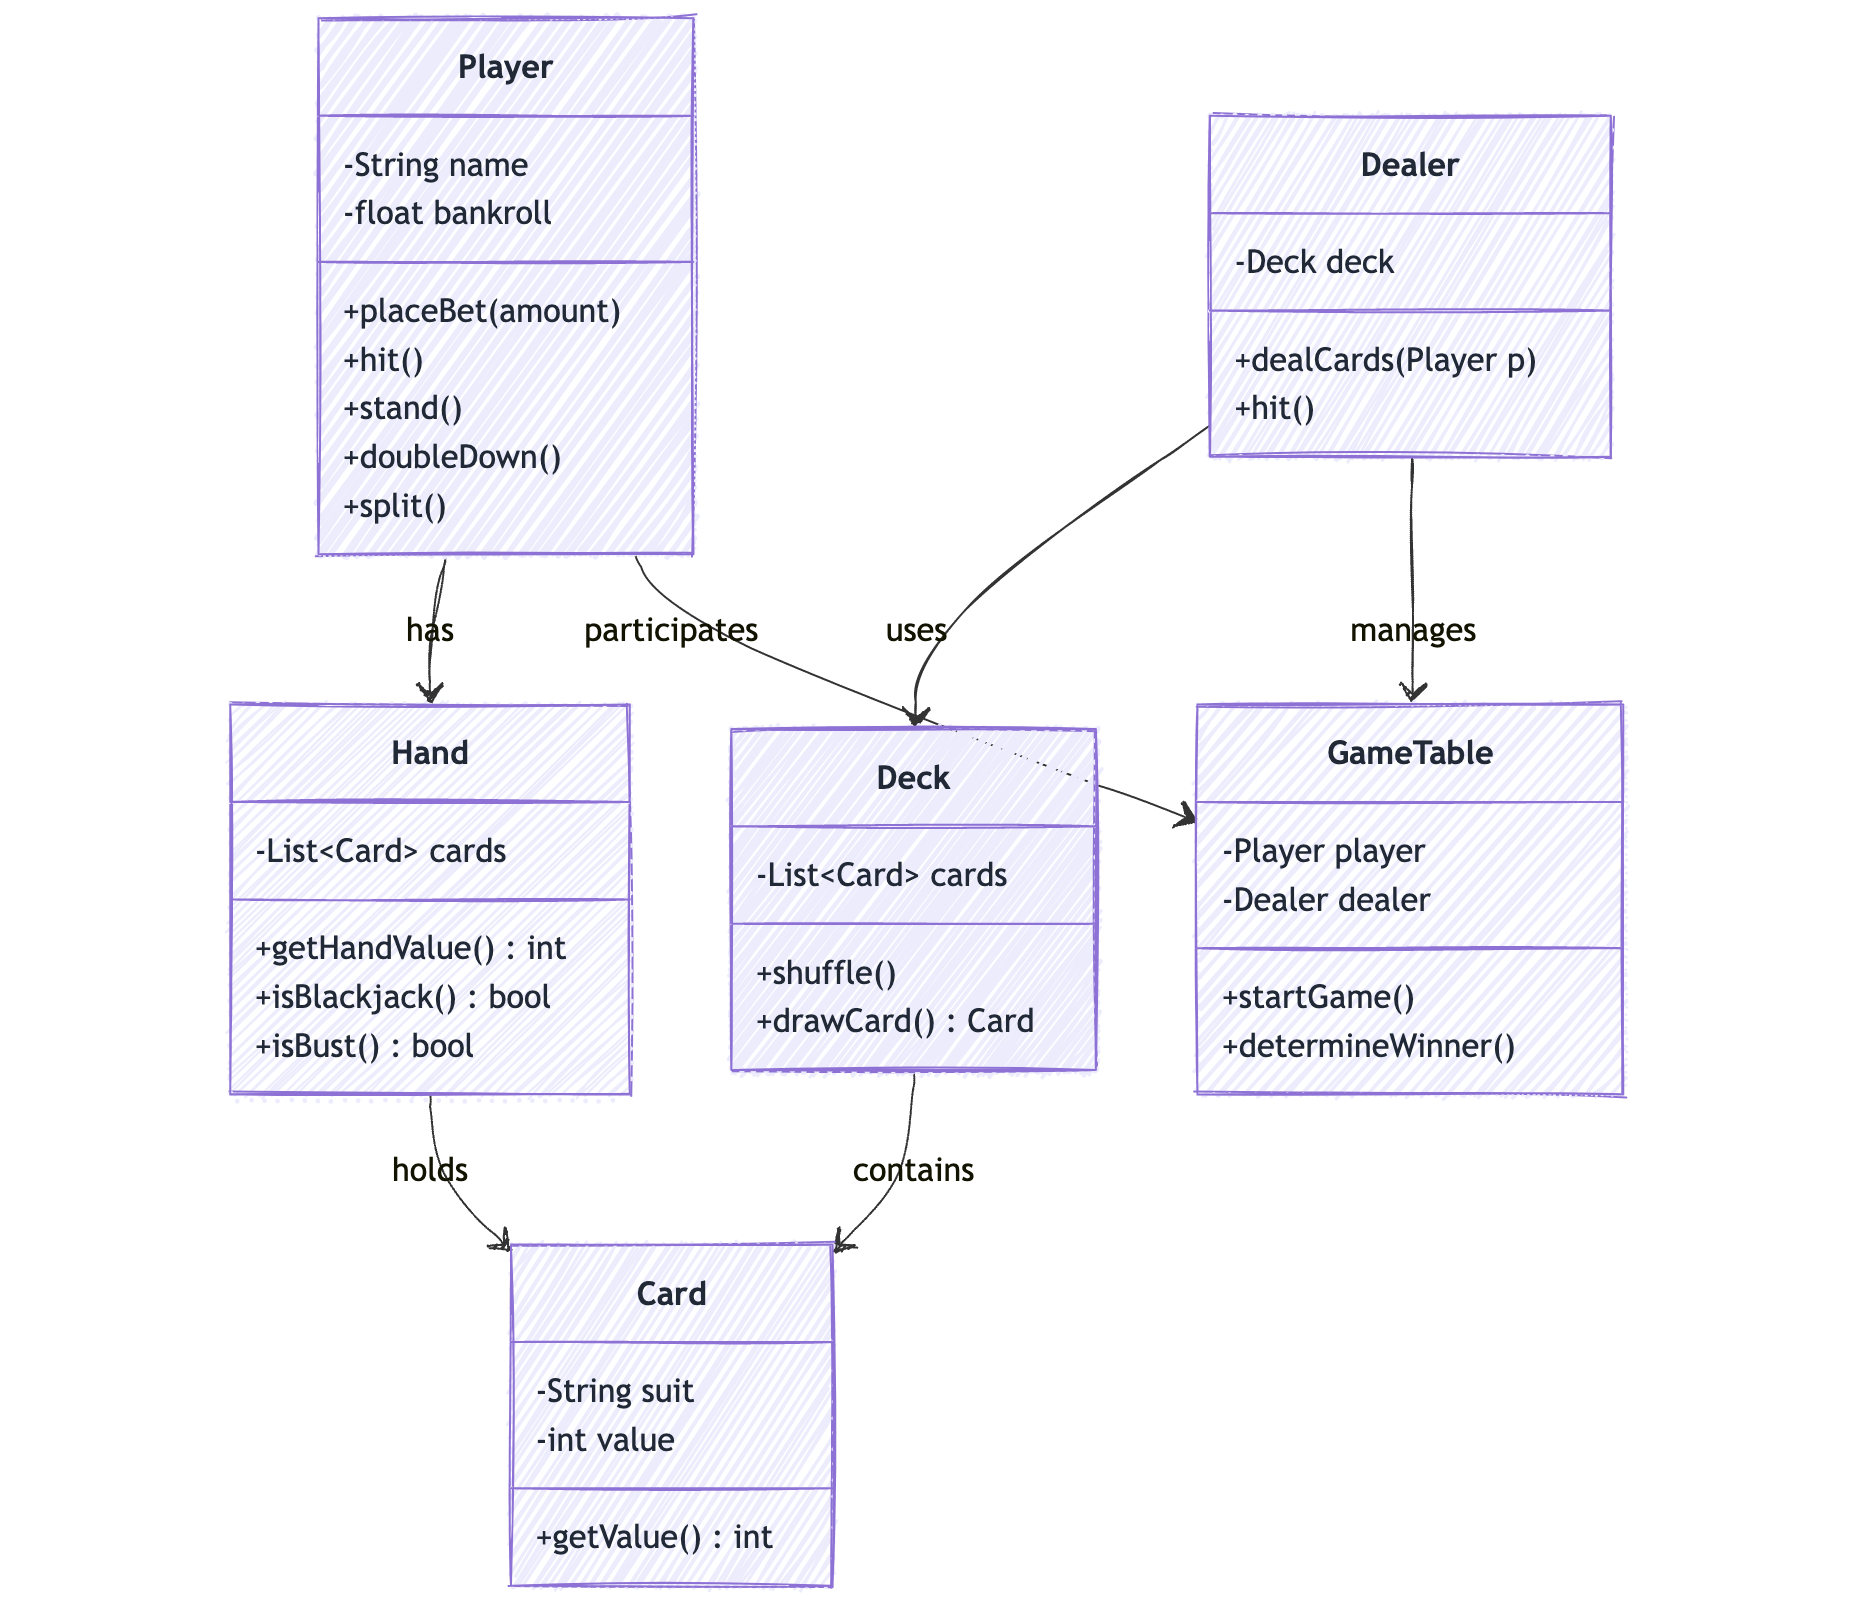
\includegraphics[scale=0.55]{report/img/classDiagram.png}
    \caption{Diagramma delle classi}
    \label{fig:classDiagram}
\end{figure}

\section{Interaction}

\begin{figure}[!htb]
    \centering
    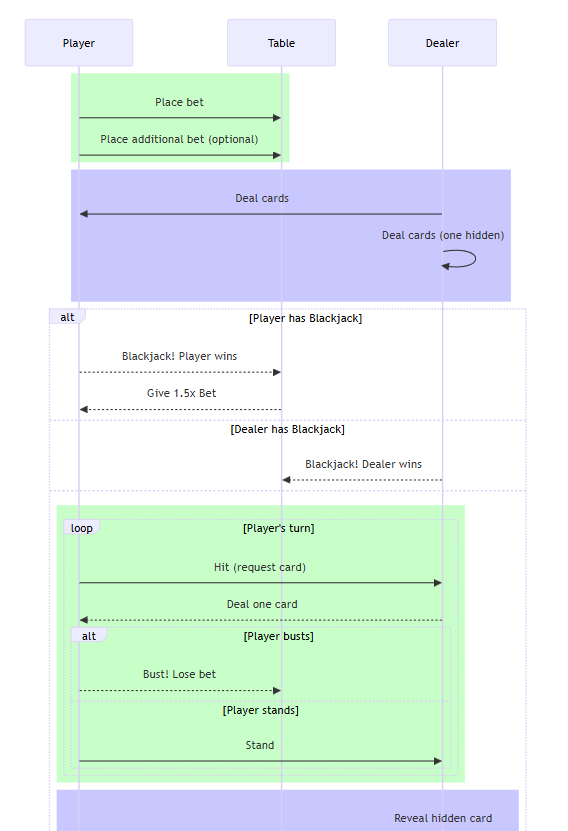
\includegraphics[scale=0.55]{report/img/sequenceDiagram.png}
    \label{fig:classDiagram}
\end{figure}
\begin{figure}[!htb]
    \centering
    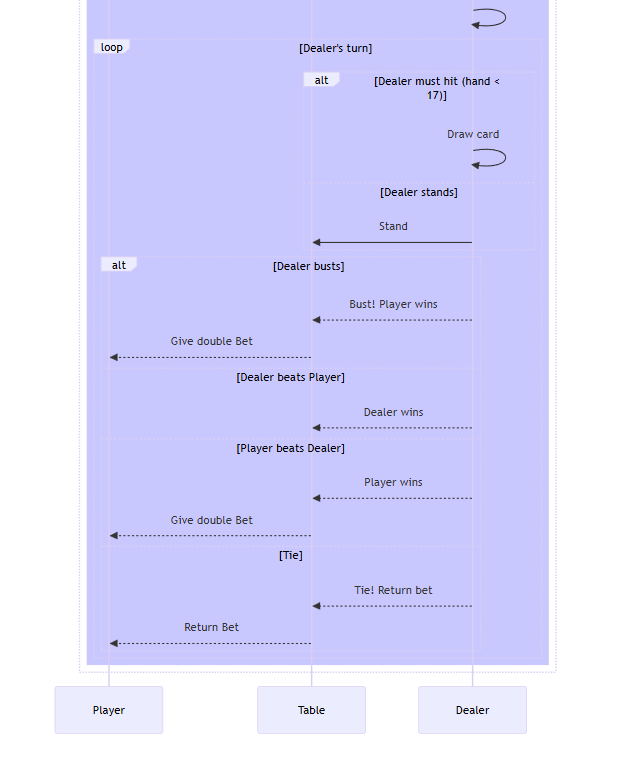
\includegraphics[scale=0.55]{report/img/sequenceDiagram2.png}
    \caption{Diagramma delle classi}
    \label{fig:classDiagram}
\end{figure}

\begin{figure}[!htb]
    \centering
    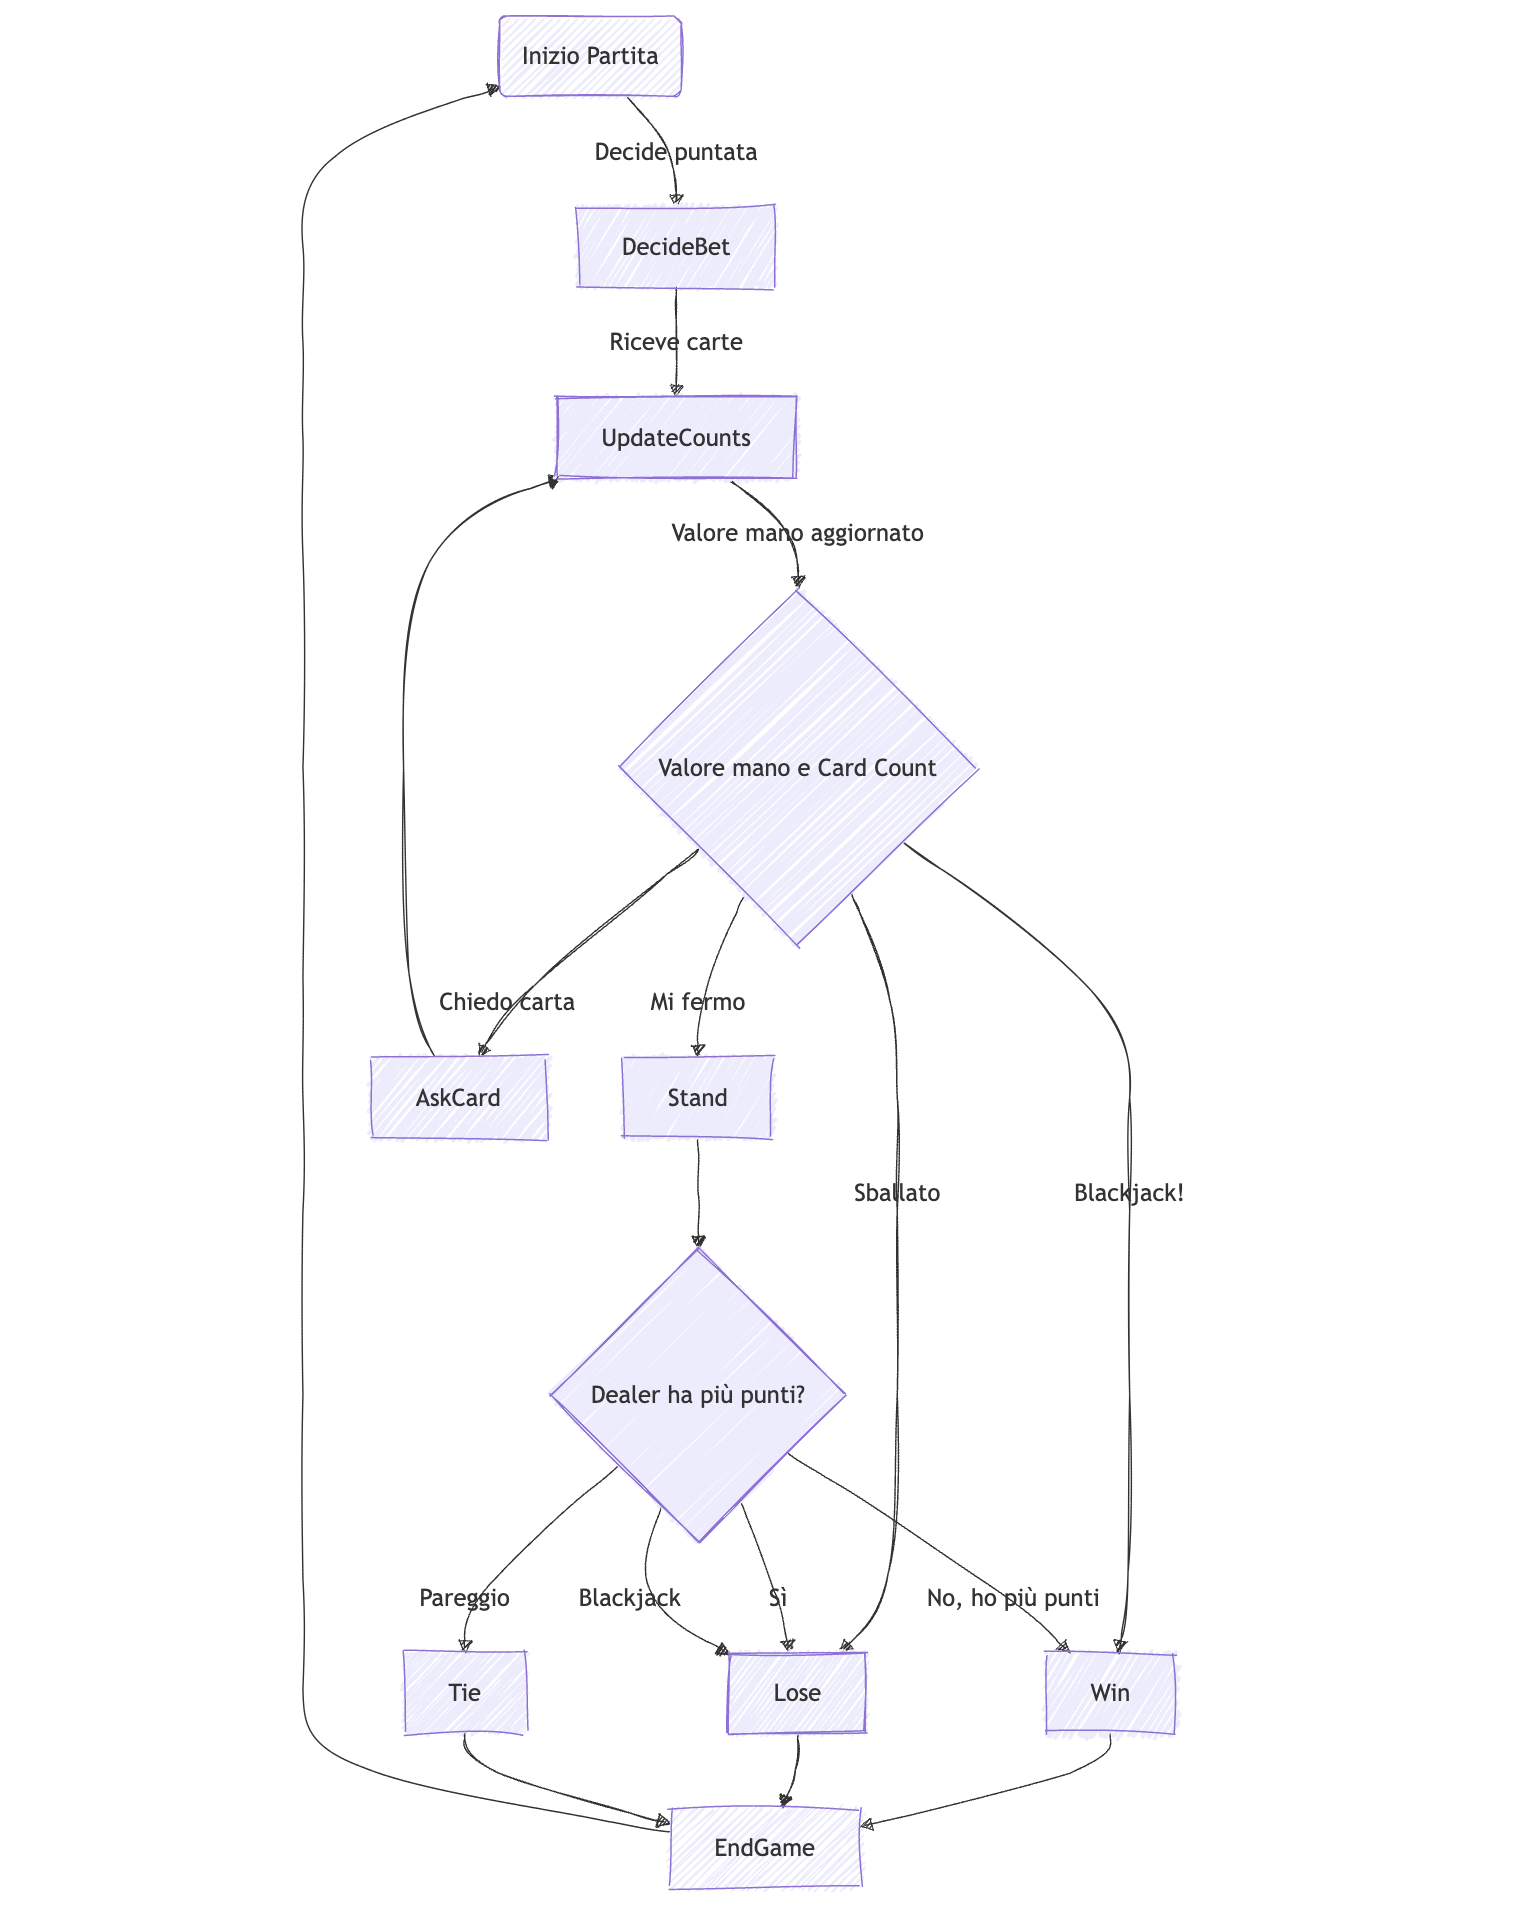
\includegraphics[scale=0.55]{report/img/activityDiagram.png}
    \caption{Diagramma delle attività}
    \label{fig:activityDiagram}
\end{figure}


\section{Architecture}
% How are software pieces organised into software modules? UML component / package /
% deployment diagrams, data-flow among components, web API description.

The project follows the basic guidelines of the MAS architecture. The more complex case of study in which an agent player relies on strategist agents has been moved to a specifc package inside the asl directory. Noteworthy is the implementation of the TwentyOneEnvironment that is used for all the case studies, to support and divide the responsability a GameEnvironmentUtils has been made to mantain a cleaner code to handle the action and beliefs of the agents. Attention has been given to some functionalities that are needed only in certain scenarios. For example the strategist agents only have to know the cards of the player only at the end of the game to update their card count when in the other circumstances player updates his internal counter in real time when sees dealer cards or hits.

\begin{lstlisting}[style=java, caption=Java implementation of different behaviour based on specifc agent, label=lst:java_stand_action]
    if("stand".equals(act)) {
        this.appWindow.actionPerformed(GameCommand.STAND);
        GameEnvUtils.checkBusted(this, agName, this.gamePanel.getDealer());
        final List<Integer> cardSeenValues = new ArrayList<>();
        // aggiunto le carte del dealer
        cardSeenValues.addAll(this.gamePanel.getDealer().hand.stream().map(Card::getValue).collect(Collectors.toList()));
        if(!"waysmarterplayer".equals(agName) && !"smartplayer".equals(agName)){
            //aggiungo anche le carte del giocatore a fine mano
            cardSeenValues.addAll(this.gamePanel.getPlayer().hand.stream().map(Card::getValue).collect(Collectors.toList()));
        }
        GameEnvUtils.sendToAgentHandToCount(this, agName, cardSeenValues);
        return true;
    }
\end{lstlisting}


\chapter{Salient implementation details}
Anything potentially interesting / non-trivial and technologies adopted to match the
design. This section is expected to be short in case some documentation (e.g. Javadoc
or Swagger Spec) has been produced for the software artefacts. This this case, the
produced documentation should be referenced here.

The approach to solve the goal of creating agents more and more capable of playing was to create each agent smarter than the one before.

\section{Smart "Novice" Agent}
First approach player only know the guidelines of the game and tries to stand below a fixed score and bet always the minium wage. The smart player is defined more or less by the routine of the game and doesn't care about the cards appeared.

\section{Way Smarter Agent}
Agent capable or memorize each card appeared on the table, both his and dealer's card contribute to alterate his perceptions and modify his behaviour on behalf of a simple strategy, the HiLo.
Keeping a conservative attitude of staying around the 18 points in hand the HiLo agents tries to overcome the dealer and have a dynamic behaviour following this idea:

\begin{itemize}
    \item If the count is \textbf{high} (\texttt{card\_count > 2}), it means there are many high cards in the deck, so we can choose to stand earlier.
    \item If the count is \textbf{low} (\texttt{card\_count < -2}), the deck is full of low cards, so we can take the risk of hitting even with a higher hand.
\end{itemize}

\begin{lstlisting}[language=Prolog]
    +hand_value(V) : ?card_count(C) & V < (18 - C) <-
    !debug_print(["Valore mano: ", V, " | Card Count: ", C, " => Chiedo carta!"]);
    !ask_card.
\end{lstlisting}

\section{Consensuos}

A facade player is at the table in the meanwhile he has a way of comunicate with some other agents that are specialized in differente strategiests of counting cards, after each hand he comunicates both his and dealer's hand to them so that they can update their inner count of cards and advice him what to do.

\subsection{Card Counting Method: ``HiLo''}

You have already mentioned the HiLo (High-Low) method, which is one of the most widely used systems. In this system, cards are assigned the following values:

\begin{itemize}
    \item Cards from 2 to 6 are worth +1
    \item Cards from 7 to 9 are neutral (0)
    \item Cards 10, J, Q, K, and A are worth -1
\end{itemize}

The count helps determine when there are more high cards (10, J, Q, K, A) in the deck, which favors the player, and when the deck is favorable to the dealer.

\subsection{Card Counting System: ``Zen Count''}

This is another counting system similar to HiLo but more complex. In this case, cards are assigned different values:

\begin{itemize}
    \item 2-3-4-5-6 = +1
    \item 7-8 = 0
    \item 9 = -1
    \item 10-J-Q-K-A = -2
\end{itemize}

This system aims to improve counting accuracy but requires more attention and skill. It tends to be more precise than HiLo in certain scenarios but is more difficult to master.

\subsection{System ``Omega II''}

The Omega II system is more complex and combines different card counting approaches. The cards are assigned the following values:

\begin{itemize}
    \item 2-3 = +1
    \item 4-5-6 = +2
    \item 7 = +1
    \item 8 = 0
    \item 9 = -1
    \item 10-A = -2
\end{itemize}

This system provides greater accuracy compared to simpler systems such as HiLo and KO, but it can be more challenging to apply due to its complexity.

Each agent then comunicates his suggested Bet and Stopping score, once the player has all the informations he choses who trust and fllows his guidelines. 

\begin{lstlisting}[language=Prolog]
    +suggest_bet(G) <-  
        ?card_count(C);
        .wait(400);
        .print("Card  count vale: ", C);
        if (C > 2) { Bet = 100; Stop = 19 } 
        if (C < -1) { Bet = 10; Stop = 16 } 
        if (C >= -1 & C <= 2) { Bet = 25; Stop = 18 }
        .print("Suggerisco di puntare: ", Bet, " e di fermarsi a: ", Stop);
        .send(advicedPlayer, tell, suggested_bet(Bet, Stop)).
\end{lstlisting}

\section{Async Agents}



% \chapter{Validation}
% Choose a criterion for the evaluation of the produced software and its compliance
% to the requirements above. Description of automated (and manual) tests and their
% rationale. In case of a test-driven development, describe tests here and possibly report
% the amount of passing tests, the total amount of tests and, possibly, the test coverage.

\chapter{Deployment Instructions}

The software has quite a simple deployment, a gradle application is used to build and run all the case studied. Running the following commands will allow to test rispectively
\begin{itemize}
    \item the "Smart" Agent.
    \item the waySmarterPlayer counting cards.
    \item the centralized strategic group of agents
\end{itemize}



\begin{lstlisting}[style=gradlestyle, caption=Runnable tasks, label=lst:bash_tasks]
    Run tasks
    ---------
    runsmartPlayerMAS - Esegue il MAS smartPlayer.mas2j
    runStrategistMAS - Esegue il MAS Strategist.mas2j
    runwaySmarterPlayerMAS - Esegue il MAS waySmarterPlayer.mas2j
\end{lstlisting}

\chapter{Conclusions}
Recap what you did.